\documentclass{beamer}
\usepackage{hyperref}
\usepackage{parskip}
\usepackage{verbatim}
\usepackage{tabularx}
% \usetheme{Madrid}
\usetheme{Boadilla}
% \usetheme{Montpellier}
\usepackage{Sweave}
\begin{document}
\Sconcordance{concordance:Lecutre_1.2.tex:Lecutre_1.2.Rnw:%
1 8 1 1 0 1805 1}


\title{R BootCamp Lecture 1.2}
\author{Steve Pittard ticopittard@gmail.com}
\subtitle{Pittard Consulting}
\date{\today}

\maketitle

% Section Variables

\section{Variables}

\begin{frame}[fragile]
\frametitle{Variables}
Everything in R is an object, which has a type and belongs to a class. There are functions that will help you figure out what it is you are working with
\small
\begin{verbatim}
3+5
[1] 8

typeof(3)
[1] "double"

class(3)
[1] "numeric"

typeof(`+`)
[1] "builtin"

\end{verbatim}
\end{frame}

%

\begin{frame}[fragile]
\frametitle{str}
The \textbf{str} function  does a really good job of telling you what the type and structure of an object is. Use it frequently ! (I do).
\newline
\scriptsize
\begin{verbatim}
myvec <- 1:10

str(myvec)
 int [1:10] 1 2 3 4 5 6 7 8 9 10
 
str(mtcars)
'data.frame':  32 obs. of  11 variables:
 $ mpg : num  21 21 22.8 21.4 18.7 18.1 14.3 24.4 22.8 19.2 ...
 $ cyl : num  6 6 4 6 8 6 8 4 4 6 ...
 $ disp: num  160 160 108 258 360 ...
 $ hp  : num  110 110 93 110 175 105 245 62 95 123 ...
 $ drat: num  3.9 3.9 3.85 3.08 3.15 2.76 3.21 3.69 3.92 3.92 ...
 $ wt  : num  2.62 2.88 2.32 3.21 3.44 ...
 $ qsec: num  16.5 17 18.6 19.4 17 ...
 $ vs  : num  0 0 1 1 0 1 0 1 1 1 ...
 $ am  : num  1 1 1 0 0 0 0 0 0 0 ...
 $ gear: num  4 4 4 3 3 3 3 4 4 4 ...
 $ carb: num  4 4 1 1 2 1 4 2 2 4 ...
\end{verbatim}
\end{frame}

% SUBSECTION NUMERIC

\subsection{Numeric}
\begin{frame}[fragile]
\frametitle{Variables}
There are four primary variable classes: numeric, character, dates, and factors. First we will look at numeric data types.

\scriptsize

\begin{verbatim}
var1 <-3

var1
[1] 3

sqrt(var1)
[1] 1.732051

var1 <- 33.3

str(var1)
[1] num 33.3

var1 + var 1
[1] 66.6

var1 * var1
[1] 1109

\end{verbatim}
\end{frame}

\begin{frame}[fragile]
\frametitle{Variables}
There is a difference between real and integer values. If you have programmed in strongly typed languages before coming to R it is important to know.

\small

\begin{verbatim}
aa <- 5

str(aa)
[1] num 5
 
aa <- as.integer(aa)

str(aa)
 int 5

aa <- 5.67

as.integer(aa)
[1] 5
\end{verbatim}
\end{frame}

% CHARACTER 
\subsection{Character}
\begin{frame}[fragile]
\frametitle{Variables}
Character strings usually represent qualitative variables. Many R functions will usually convert character variables into factors if necessary but not always. (We will discuss factors soon enough) 
 

\footnotesize
\begin{verbatim}
var.one <- "Hello there ! My name is Steve."

var.two <- "How do you do ?"

var.one
[1] "Hello there ! My name is Steve."

nchar(var.one) # Number of characters present
[1] 31

toupper(var.one)
[1] "HELLO THERE ! MY NAME IS STEVE."

\end{verbatim}
\end{frame}

\begin{frame}[fragile]
\frametitle{Variables}
Character strings usually represent qualitative variables. Many R functions will usually convert character variables into factors if necessary but not always. (We will discuss factors soon enough) 
\newline
\footnotesize
\begin{verbatim}
mydna <- c("A","G","T","C","A")

str(mydna)
chr [1:5] "A" "G" "T" "C" "A"

mydna
[1] "A" "G" "T" "C" "A"

pi <- "3.14"
str(pi)
 chr "3.14"
 
pi + pi
Error in pi + pi : non-numeric argument to binary operator
\end{verbatim}
\end{frame}

\begin{frame}[fragile]
\frametitle{Variables}
\footnotesize
\begin{verbatim}
paste(var.one, var.two)
[1] "Hello there ! My name is Steve. How do you do ?"

paste(var.one, var.two, sep=":")
[1] "Hello there ! My name is Steve.:How do you do ?"

strsplit(var.one, " ")
[[1]]
[1] "Hello" "there" "!" "My" "name" "is" "Steve."

patientid <- "ID:011472:M:C" # Encodes Birthday, Gender, and Race

strsplit(patientid, ":")
[[1]]
[1] "ID" "011472" "M" "C"

bday <- strsplit(patientid, ":")[[1]][2] # Get just the birthday

\end{verbatim}
\end{frame}


% SUBSECTION DATES

\subsection{Dates}

% Sys.Date

\begin{frame}[fragile]
\frametitle{Dates}
R has a builtin function called Sys.Date() that can tell you the date. It looks like it returns just a character string but it returns a true date object. (Use \textbf{str} when in doubt). But Sys.Date() doesn't help us convert strings to dates. 
\newline
\begin{verbatim}
Sys.Date()
[1] "2014-12-05"

Sys.Date() + 1
[1] "2014-12-06"

str(Sys.Date())
 Date[1:1], format: "2014-12-05"
\end{verbatim}
\end{frame}

% Sys.Date

\begin{frame}[fragile]
\frametitle{Dates}
So unless you tell R that a string is in fact a ``real'' date it will assume that it is simply a character string.  
\footnotesize
\begin{verbatim}
somedate <- "03/17/99"

str(somedate)
 chr "03/17/99"

somedate+1
Error in somedate + 1 : non-numeric argument to binary operator

realdate <- as.Date("03/17/99","%m/%d/%y")

str(realdate)
 Date[1:1], format: "1999-03-17"

realdate+1
[1] "1999-03-18"
\end{verbatim}
\end{frame}


\begin{frame}[fragile]
\frametitle{Dates}
R has multiple functions and packages to handle dates which can be confusing to the newcomer. The following chart attempts to summarize them and present their respective capabilities.
\newline
\begin{center}
\begin{tabular}{| l | l || c | c | c |}
  \hline         
  Function & Package & Dates & Times & Timezones \\ \hline
  as.Date() & Base & Y & N & Y  \\ \hline
  chron & chron & Y & Y & N \\ \hline
  POSIX & Base & Y & Y & Y \\ \hline
  lubridate & lubridate & Y & Y & Y \\ 
  \hline  
\end{tabular}
\end{center}

The rule of thumb is to use the function that satisfies the need. So if you need to convert just dates and no times then use as.Date(). If you need date, time, and timezone support then use POSIX tools or lubridate.
\end{frame}


\begin{frame}[fragile]
\frametitle{as.Date()}
The \textbf{as.Date()} function handles dates involving years, months, and days. It does not handle times. It is easy to use once you learn the tokens.

\small
\begin{verbatim}
as.Date("January 01 2010","%b %d %Y")
[1] "2010-01-01"

as.Date("Jan 01, 2010","%b %d, %Y")
[1] "2010-01-01"

as.Date("01/01/10","%m/%d/%y")
[1] "2010-01-01"

as.Date("1Jan2010","%d%b%Y")
[1] "2010-01-01"
\end{verbatim}
\end{frame}


\begin{frame}[fragile]
\frametitle{as.Date()}
The \textbf{as.Date()} function handles dates involving years, months, and days. It does not handle times. It is easy to use once you learn the tokens. 
\newline
\begin{center}
\begin{tabular}{| l | l | }
  \hline         
  Token & Value \\ \hline
  \%d & Day of the month (decimal number) \\ \hline
  \%m & Month (decimal number) \\ \hline
  \%b & Month (abbreviated) \\ \hline
  \%B & Month (full name) \\ \hline
  \%y & Year (2 digit) \\ \hline
  \%Y & Year (4 digit) \\ \hline
  \hline  
\end{tabular}
\end{center}
\end{frame}

\begin{frame}[fragile]
\frametitle{as.Date()}
Once dates have been converted we can perform arithmetic and logical operations on them. 
\footnotesize
\begin{verbatim}
date1 <- as.Date("03/17/08","%m/%d/%y")

date2 <- as.Date("04/17/08","%m/%d/%y")

date2 - date1
Time difference of 31 days

mean(c(date1,date2))
[1] "2008-04-01"

date2 < date1
[1] FALSE

date2 > date1
[1] TRUE
\end{verbatim}
\end{frame}


\begin{frame}[fragile]
\frametitle{as.Date()}
This function can help us convert columns in a data frame that contain dates as character strings
\footnotesize
\begin{verbatim}
mydf <- data.frame(measure=round(rnorm(4),2),date=c("01/23/01",
                     "02/20/01","02/22/01","03/04/01"))
str(mydf)
'data.frame':  4 obs. of  2 variables:
 $ measure: num  1.03 -0.46 -1.56 -0.65
 $ date   : Factor w/ 4 levels "01/23/01","02/20/01",..: 1 2 3 4

mydf$date
[1] 01/23/01 02/20/01 02/22/01 03/04/01
Levels: 01/23/01 02/20/01 02/22/01 03/04/01

mydf$date <- as.Date(mydf$date,"%m/%d/%y")
str(mydf$date)
 Date[1:4], format: "2001-01-23" "2001-02-20" "2001-02-22" "2001-03-04"
\end{verbatim}
\end{frame}


\begin{frame}[fragile]
\frametitle{as.Date()}
There are some helper functions that make it easy to figure out the month name of a series of dates or whether a given date represents a weekday.  
\footnotesize
\begin{verbatim}
months(mydf$date)
[1] "January"  "February" "February" "March"   

weekdays(mydf$date)
[1] "Tuesday"  "Tuesday"  "Thursday" "Sunday"  

quarters(mydf$date)
[1] "Q1" "Q1" "Q1" "Q1"

table(months(mydf$date))
February  January    March 
       2        1        1 
\end{verbatim}
\end{frame}


% STRPTIME

\begin{frame}[fragile]
\frametitle{strptime}
In general I prefer to use the POSIX tools to work with dates. The primary function is strptime.
\footnotesize
\begin{verbatim}
strptime("1945-11-04","%Y-%m-%d")
[1] "1945-11-04 EST"
 
strptime("Tuesday March 17, 2011 01:10:05","%A %B %d, %Y %H:%M:%S")
[1] "2011-03-17 01:10:05 EDT"

strptime("11/14/45 10:10:00 AM","%m/%d/%y %I:%M:%S %p")
[1] "2045-11-14 10:10:00 EST"

strptime("11/14/45 10:10:00 PM","%m/%d/%y %I:%M:%S %p")
[1] "2045-11-14 22:10:00 EST"

\end{verbatim}
\end{frame}

\begin{frame}[fragile]
\frametitle{strptime}
\footnotesize
\begin{verbatim}
date1 <- strptime("11/14/45 10:10:00 AM","%m/%d/%y %I:%M:%S %p")

date2 <- strptime("11/14/45 10:10:00 PM","%m/%d/%y %I:%M:%S %p")

date2 - date1
Time difference of 12 hours

# Same as 

difftime(date2,date1)
Time difference of 12 hours

# We can convert many dates at once 

strptime(c("03/27/2003","03/27/2003","04/14/2008"),format="%m/%d/%Y")
[1] "2003-03-27 EST" "2003-03-27 EST" "2008-04-14 EDT"
\end{verbatim}
\end{frame}

\begin{frame}[fragile]
\frametitle{strptime}
Since strptime handles times as well as dates you will need to know the tokens necessary to process times. The tokens to process dates are the same as with as.Date()
\footnotesize

\begin{tabular}{| l | l || l | l |}
  \hline         
  Token & Meaning & Token & Meaning \\ \hline
  \%a & Abbreviated weekday & \%A & Full weekday \\ 
  \%b & Abbreviated Month & \%B & Full month \\ 
  \%c & Locale-specific date and time & \%d & Decimal Date \\
  \%H & Decimal hours (24 hr) & \%I & Decimal hours (12 hr) \\
  \%j & Decimal day of yr & \%m & Decimal month \\
  \%M & Decimal minute & \%p & Locale-specific AM/PM \\
  \%S & Decimal second & \%U & Decimal week of yr (Sunday) \\
  \%w & Decimal wkday (0=Sunday) & \%W & Decimal week of yr (Monday) \\
  \%x & Locale-specific date & \%X & Locale-specific time \\
  \%y & 2-digit year & \%Y & Locale-specific time \\
  \%z & Offset from GMT & \%Z & Time zone (character) \\ 
  \hline  
\end{tabular}
\end{frame}

\begin{frame}[fragile]
\frametitle{strptime}
We can also easily generate sequences of dates if necessary.
\newline
\scriptsize
\begin{verbatim}
start_date <- strptime('01/10/2011','%m/%d/%Y')

seq(start_date,by=5,length=3)
[1] "2011-01-10 00:00:00 EST" "2011-01-10 00:00:05 EST" "2011-01-10 00:00:10 EST"

date1 <- strptime('01/10/2011','%m/%d/%Y')

date2 <- strptime('02/01/2011','%m/%d/%Y')

seq(date1,to=date2,by='1 week')
[1] "2011-01-10 EST" "2011-01-17 EST" "2011-01-24 EST" "2011-01-31 EST"
 
\end{verbatim}
\end{frame}

\begin{frame}[fragile]
\frametitle{Picking a Date Apart}
Once we have a date we can access ``parts'' of it
\newline
\footnotesize
\begin{verbatim}
mydate <- strptime("12/11/2014 05:15:00","%m/%d/%Y %H:%M:%S")

str(mydate)
POSIXlt[1:1], format: "2014-12-11 05:15:00"

ls(mydate)
[1] "gmtoff" "hour"   "isdst"  "mday"   "min"    "mon"    "sec"    
     "wday"  "yday"  "year"   "zone"  

mydate$hour
[1] 5

mydate$wday
[1] 4

\end{verbatim}
\end{frame}


\begin{frame}[fragile]
\frametitle{Picking a Date Apart}
Once we have a date we can re format it to suit our needs without changing the underlying date
structure.
\footnotesize
\begin{verbatim}
mydate <- strptime("12/11/2014 05:15:00","%m/%d/%Y %H:%M:%S")
 
format(mydate,'%Y')   # 4 digit year
[1] "2014"

format(mydate,'%b')   # Abbreviated month name
[1] "Dec"

format(mydate,'%B')   # Full month name
[1] "December"

format(mydate,'%W')   # Numeric week of the year
[1] "49"

format(mydate,'%w')   # Numeric day of the week (Sunday = 0)
[1] "4"

\end{verbatim}
\end{frame}

% SUBSECTION LOGICALS

\begin{frame}[fragile]
\frametitle{Logical}
Logical variables are those that take on a TRUE or FALSE value. Either by direct assignment or as the
result of some comparison:
\footnotesize
\begin{verbatim}
some.variable < TRUE
some.variable
[1] TRUE

some.variable <- (4 < 5)
some.variable 
[1] TRUE
\end{verbatim}
\normalsize
Note that the following is equivalent to the above. Enclosing an R statement  within parenthesis will print out the value of that statement.
\footnotesize
\begin{verbatim}
(some.variable <- (4 < 5 ))
[1] TRUE
\end{verbatim}
\end{frame}

\begin{frame}[fragile]
\frametitle{Logical}
Logicals are extremely important especially when using if-statements as part of writing functions. 
\begin{verbatim}
if (some_logical_condition) {
    do something
} else {
    do something else
}

if (4 < 5) {
  print("Four is less than Five")
}
\end{verbatim}
\end{frame}


\begin{frame}[fragile]
\frametitle{Logical}
Logicals are extremely important especially when using if-statements as part of writing functions. 
\small
\begin{verbatim}
my.var <- ( 4 < 5)

if (my.var) {
    print("four is less than five")
}
[1] "four is less than five"

if (! my.var ) {
    print("four is greater than five")
}

\end{verbatim}
\end{frame}

\begin{frame}[fragile]
\frametitle{Logical}
We use logical operators to link smaller comparisons. For example, the \& character is the logical AND operator.

In the following statement both expressions on either side of the AND operator need to be TRUE for my.var to be TRUE.

\small
\begin{verbatim}
my.var <- (4 < 5) & (4 < 6) # & is the "AND" operator
my.var
[1] TRUE
\end{verbatim}
\normalsize

The logical OR operator is the | character. Only one of the expressions on either side of the OR operator needs to be TRUE for my.var to be TRUE
\small
\begin{verbatim}
my.var <- (4 < 5) | ( 4 < 6 ) # Logical OR operator
my.var
[1] TRUE
\end{verbatim}
\end{frame}

% SECTION INTERROGATION/COERCION

\section{Interrogation/Coercion}
\begin{frame}[fragile]
\frametitle{Interrogation/Coercion}
It is commont to interrogate variables from within some programming logic to see what they are (or are not). It is also common to ``coerce'' variables into another form. There are functions for both activities.
\newline
\begin{center}
\begin{tabular}{| l | l | }
  \hline         
  Interrogation & Coercion \\ \hline
  is.array() & as.array() \\ 
  is.character() & as.character() \\ 
  is.date.frame() & as.data.frame \\ 
  is.factor() & as.factor() \\ 
  is.list() & as.list() \\ 
  is.logical() & as.logical() \\ 
  is.matrix() & as.matrix() \\
  is.numeric() & as.numeric() \\ 
  is.vector() & as.vector() \\
  \hline  
\end{tabular}
\end{center}
\end{frame}

\begin{frame}[fragile]
\frametitle{Interrogation/Coercion}
Here are some examples of interrogation:
\begin{verbatim}
pi <- 3.14

is.integer(pi)
[1] FALSE

is.numeric(pi)
[1] TRUE

is.character(pi)
[1] FALSE

is.logical(pi)
[1] FALSE
\end{verbatim}
\end{frame}

\begin{frame}[fragile]
\frametitle{Interrogation/Coercion}
Here are some examples of coercion. We coerce variables usually after we read in some data but we also do it when writing functions to process data frames.
\newline
\begin{verbatim}
pi <- 3.14

as.integer(pi)
[1] 3

as.character(pi)
[1] "3.14"

as.numeric(as.character(pi))
[1] 3.14
\end{verbatim}
\end{frame}

\begin{frame}[fragile]
\frametitle{Interrogation/Coercion}
Here we use both interrogation and coercion to check arguments to a function that computes the mean of a vector.
\newline
\scriptsize
\begin{verbatim}
mymean <- function(x) {
#
# Function to compute the mean of a numeric vector
#
  if (!is.vector(x)) {
    stop("The argument is not a vector")
  }
  if (!is.numeric(x)) {
      print("The arguement is not numeric - Trying to convert to numeric")
      x <- as.numeric(x)
  }   
  return(sum(x)/length(x))
}

mymean(c("1","2","3","4"))
[1] "The arguement is not numeric - Trying to convert to numeric"
[1] 2.5
\end{verbatim}
\end{frame}

\section{vectors}
\begin{frame}[fragile]
\frametitle{Vectors}
Vectors are a fundamental data structure in R. It is absolutely essential that you know how to be 
productive using vectors. Vectors can have the types described previously, (integer, logical,real, character, factor).
\newline
\footnotesize
\begin{verbatim}
1:10

rnorm(10)

y <- 5.4 # A single assignment

y <- 1:10 # A vector with 10 elements (1 .. 10)

y <- c(1,2,3,4,5,6,7,8,9,10) # Same as above yet using the "c" function

y <- scan() # Allows you to enter in elements from the keyboard
1: 10
2: 9
3: 8
..
1: 1
\end{verbatim}
\end{frame}

\begin{frame}[fragile]
\frametitle{Vectors}
Let's say we have measured the heights of some people. Vectors are perfect for stashing this info.
Also - \textbf{Bracket Notation} is the key to working with vectors.
\newline
\scriptsize
\begin{verbatim}
height <- c(59,70,66,72,62,66,60,60) # create a vector of 8 heights

height[1:5] # Get first 5 elements
[1] 59 70 66 72 62

height[5:1] # Get first 5 elements in reverse
[1] 62 72 66 70 59

height[-1] # Get all but first element
[1] 70 66 72 62 66 60 60

height[-1:-2] # Get all but first two elements
[1] 66 72 62 66 60 60

height[c(1,5)] # Get just first and fifth elements
[1] 59 62
\end{verbatim}
\end{frame}

\begin{frame}[fragile]
\frametitle{Vectors}
If we have a vector we can apply logical tests. This is very powerful
\newline
\footnotesize
\begin{verbatim}
height
[1] 59 70 66 72 62 66 60 60

height == 72 # Test for values equal to 72
[1] FALSE FALSE FALSE TRUE FALSE FALSE FALSE FALSE

height[height == 72]
[1] 72

# SAME AS
logical.vector <- (height == 72)
logical.vector
[1] FALSE FALSE FALSE TRUE FALSE FALSE FALSE FALSE

height[ logical.vector ]
\end{verbatim}
\end{frame}

\begin{frame}[fragile]
\frametitle{Vectors}
There are operators we can use to combine logical comparisons
\newline
\footnotesize
\begin{verbatim}
# Note use of the "&" / and operator

height[height > 60 & height < 70]
66 62 66

height[height > 60 & height <= 70]
70 66 62 66

height[height < 60 | height > 70]
[1] 59 72

> height[(height < 60) | (height > 70)]  
[1] 59 72
\end{verbatim}
\end{frame}


\begin{frame}[fragile]
\frametitle{Vectors}
Vectors exist, in part, to help us avoid having t o write ``for loops'' everytime we want to process a vector and summarize it. Compare the following:
\newline
\footnotesize
\begin{verbatim}
height[height > 60 & height < 70]
66 62 66

# As opposed to this 

for (ii in 1:length(height)) {
   if (height[ii] > 60 & height[ii] < 70) {
      print(height[ii])
   }
}
66
62
66
\end{verbatim}
\end{frame}


\begin{frame}[fragile]
\frametitle{Vectors}
Let's create a weight vector that corresponds to the height vector. (We measured the same people)
\newline
\footnotesize
\begin{verbatim}
weight <- c(117,165,139,142,126,151,120,166) # weight (in lbs)

weight/100
[1] 1.17 1.65 1.39 1.42 1.26 1.51 1.20 1.66

sqrt(weight)
[1] 10.81665 12.84523 11.78983 11.91638 11.22497 12.28821 10.95445 12.88410

weight^2
[1] 13689 27225 19321 20164 15876 22801 14400 27556

sum((weight-mean(weight))^2)/(length(weight)-1) # The variance formula
[1] 363.9286

var(weight)
[1] 363.9286
\end{verbatim}
\end{frame}

\begin{frame}[fragile]
\frametitle{Vectors}
\small
\begin{verbatim}
height <- c(59,70,66,72,62,66,60,60)

weight <- c(117,165,139,142,126,151,120,166)

# Get 8 weight measurements

cor(height,weight) # Are they correlated ?
[1] 0.46295

plot(weight,height,main="Height & Weight Plot") # Do a X/Y plot

res <- lm(height ~ weight) # Do a linear regression

abline(res) # Check out the regression line
\end{verbatim}
\end{frame}

\begin{frame}[fragile]
\frametitle{Vectors}
\begin{center}
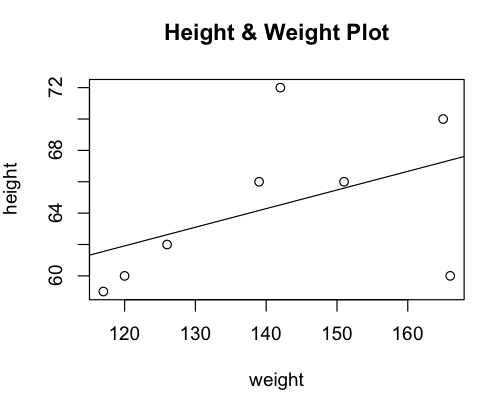
\includegraphics[width=3.6in]{/Users/fender/Dropbox/PCONS.DIR/IMG.DIR/lm.png}
\end{center}
\end{frame}

\begin{frame}[fragile]
\frametitle{Vectors}
\small
\begin{verbatim}
weight <- c(117,165,139,142,126,151,120,166) # weight (in lbs)

new.weights <- weight + 1 # Vector Addition

new.weights
[1] 118 166 140 143 127 152 121 167

append(weights,new.weights) # Combines the two vectors
[1] 117 165 139 142 126 151 120 166 118 166 140 143 127 152 121 167

c(weight,new.weights) # Equivalent to the above

round(weight/new.weights,2)
[1] 0.99 0.99 0.99 0.99 0.99 0.99 0.99 0.99
\end{verbatim}
\end{frame}

% 

\begin{frame}[fragile]
\frametitle{Vectors - Characters}
\footnotesize
\begin{verbatim}
gender <- c("F","M","F","M","F","M","F","M") # Get their gender

smoker <- c("N","N","Y","Y","Y","N","N","N") # Do they smoke ?

table(gender,smoker) # Let's count them
      smoker
gender N Y
     F 2 2
     M 3 1
     
prop.table(table(gender,smoker))
      smoker
gender N Y
     F 0.250 0.250
     M 0.375 0.125

library(lattice)

barchart(table(gender,smoker),auto.key=TRUE,main="Smoking M/F")
\end{verbatim}
\end{frame}


\begin{frame}[fragile]
\frametitle{Vectors - Characters}
\begin{center}
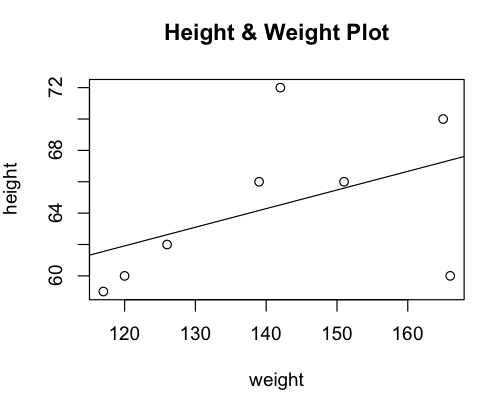
\includegraphics[width=3.6in]{/Users/fender/Dropbox/PCONS.DIR/IMG.DIR/lm.png}
\end{center}
\end{frame}

%

\begin{frame}[fragile]
\frametitle{Vectors - Characters}
An important attribute of a vector is its length. To determine its length, (or set it), one
uses the "length" function.
\footnotesize
\begin{verbatim}

y <- 1:10
length(y) # Length of the entire vector
[1] 10

vec1 <- 1:5

vec2 <- c(1,3)

vec1 + vec2 # The shorter vector (vec2) is recycled
[1] 2 5 4 7 6

Warning message:
In vec1 + vec2 :
longer object length is not a multiple of shorter object length
\end{verbatim}
\end{frame}

%

\begin{frame}[fragile]
\frametitle{Vectors - Characters}
You can name the elements of a vector. In this example, let's say we have measured some heights of
eight people.
\scriptsize
\begin{verbatim}
height <- c(59,70,66,72,62,66,60,60)

# Let's also create a character vector that contains the names of people
# whose heights we measured

my.names <- c("Jacqueline","Frank","Babette","Mario","Adriana",
              "Esteban","Carole","Louis")

names(height) <- my.names

height

Jacqueline  Frank   Babette   Mario  Adriana  Esteban   Carole  Louis 
    59       70       66        72     62       66        60      60 
\end{verbatim}
\end{frame}

%

\begin{frame}[fragile]
\frametitle{Vectors - Characters - which}
The \textbf{which} command allows us to determine which element number(s) satisfies a condition. If the element has a name then we will also see that listed.
\footnotesize
\begin{verbatim}
height > 60
[1] FALSE TRUE TRUE TRUE TRUE TRUE FALSE FALSE

which(height > 60)
Frank Babette Mario Adriana Esteban
  2      3      4      5       6

height[which(height > 60)]
Frank Babette   Mario Adriana Esteban 
  70      66      72      62      66 

# Note that the element names do not interfere with numeric evaluations

mean(height)
[1] 64.375
\end{verbatim}
\end{frame}

%

\begin{frame}[fragile]
\frametitle{Vectors - Names - paste}
The \textbf{pastes} function allows us to rapidly generate label names for a vector. For example we can rapdily generate names for observations according to a pattern.
\small
\begin{verbatim}
new.names <- paste("ID",1:8,sep="_")

new.names
[1] "ID_1" "ID_2" "ID_3" "ID_4" "ID_5" "ID_6" "ID_7" "ID_8"

names(height) <- new.names

height
ID_1 ID_2 ID_3 ID_4 ID_5 ID_6 ID_7 ID_8
 59   70   66   72  62    66   60   60
\end{verbatim}
\end{frame}

% Missing Values

\begin{frame}[fragile]
\frametitle{Vectors - Missing Values}
\small
\begin{verbatim}
gender <- c("F","M","F","M","F","M","F","M") # Get their gender

smoker <- c("N","N","Y","Y","Y","N","N","N") # Do they smoke ?

length(gender) # Gives current length of vector
[1] 8

length(gender) <- 10 # Sets length of the vector

gender # NA represents a missing value
[1] "F" "M" "F" "M" "F" "M" "F" "M" NA NA
\end{verbatim}
\end{frame}

% 
\begin{frame}[fragile]
\frametitle{Vectors - Missing Values}
\footnotesize
\begin{verbatim}
is.na(gender)
[1] FALSE FALSE FALSE FALSE FALSE FALSE FALSE FALSE TRUE TRUE

which(is.na(gender)) # Which elements contain missing values
[1] 9 10

which(!is.na(x))

# Which elements don't have missing values
[1] 1 2 3 4 5 6 7 8

gender[!is.na(gender)] # Get elements which aren't missing
[1] "F" "M" "F" "M" "F" "M" "F" "M"

gender[9:10] = "-" # Set all NAs to "-" but probably should leave NAs
[1] "F" "M" "F" "M" "F" "M" "F" "M" "-" "-"

\end{verbatim}
\end{frame}

% Some commin functions

\begin{frame}[fragile]
\frametitle{Vectors - Functions}
Here are some of the functions in R that operate on vectors. There are many, many more.
\newline

\footnotesize
\begin{tabular}{| l | l || l | l |}
  \hline         
  \textbf{Function} & \textbf{Purpose} & \textbf{Function} & \textbf{Purpose} \\ \hline
  sum(x) & Sum of x & prod(x) & Product of x  \\ \hline
  cumsum(x) & Cumulative sum & cumprod(x) & Cumulative product \\ \hline
  min(x) & Minimum value & max(x) & Maximum value \\ \hline
  mean(x) & Mean value & median(x) & Median value\\ \hline
  var(x) & Variance & sd(x) & Standard Deviation \\ \hline
  cov(x) & Covariance & cor(x) & Correlation \\ \hline
  range(x) & Range of x & quantile(x) & quantiles of x \\ \hline
  fivenum(x) & Five number summary & length(x) & Number of elements \\ \hline
  unique(x) & Gets unique elements & rev(x) & Revereses x \\ \hline
  sort(x) & Sorts x & match(x,y) & Finds position of x in y \\ \hline
  union(x,y) & Union of x and y & intersect(x,y) & Intersection of x and y \\ \hline
  setdiff(x,y) & Elements of x not in y & setequal(x,y) & Test if x and y equal \\
  \hline  
\end{tabular}
\end{frame}

% Common logical operators

\begin{frame}[fragile]
\frametitle{Vectors - Logical Operators}
\scriptsize
\begin{verbatim}
# RELATIONAL OPERATORS

Equal to               ==           if (myvar == "test") {print("EQ")} 
                       ==           if (mnynum == 3)     {print("EQ")} 
Not equal to           !=           if (myvar != "test") {print("NE")} 
Less than or equal to  <=           if (number <= 5)     {print("LTE")}
Less than              <            if (number < 10)     {print("LT")}
Greater than or equal to  >=        if (number >= 10)    {print("GTE")}
Greater than              >         if (number > 12)     {print("GT")}

# BOOLEAN OPERATORS 

And                    &      if ((myvar == "test") & (num <= 10) ) { 
                                     print("Equal and less than")
                              }
                                     
Not                    !      if (!complete.cases(myvec)) {
                                     print("Non complete cases")
                              } 

Or                     |      if ((num > 3) | (num < -3)) {
                                     print("Only one of these has to be true")
                              }
\end{verbatim}
\end{frame}

% Example functions

\begin{frame}[fragile]
\frametitle{Vectors - Various Examples}
\scriptsize
\begin{verbatim}
mean(height) # Get the mean
[1] 64.375

sd(height) # Get standard deviation
[1] 4.897157

min(height) # Get the minimum
[1] 59

range(height) # Get the range
[1] 59 72

# Tukey's summary (minimum, lower hinge, median, upper hinge, maximum)
fivenum(height) 
[1] 59 60 64 68 72

length(height) # Vector length
[1] 8

quantile(height) # Quantiles
0% 25% 50% 75% 100%
59  60  64  67  72
\end{verbatim}
\end{frame}

% More Example functions

\begin{frame}[fragile]
\frametitle{Vectors - Various Examples}
\scriptsize
\begin{verbatim}
# Generate 10000 numbers from a Normal distribution

set.seed(123)
my.vals <- rnorm(10000,20,2)   # Mean of 20 and sd of 2
 
max(my.vals)   # Find max 
[1] 27.69554

which.max(my.vals) # Which element is the max ? 
[1] 8156

my.vals[ which.max(my.vals) ]  # Confirm
[1] 27.69554

min(my.vals)    # Find min ?
[1] 12.30936

my.vals[ which.min(my.vals) ]   # Confirm
[1] 12.30936
 
x <- 1:16
x[x %% 2 == 0] # Find the even numbers between 1 and 16
[1]  2  4  6  8 10 12 14 16
\end{verbatim}
\end{frame}

% 

\begin{frame}[fragile]
\frametitle{Vectors - Various Examples}
We want to find the sum of all the elements in x that are less than 5.
\footnotesize
\begin{verbatim}
x <- 0:10

x[ x < 5 ]
[1] 0 1 2 3 4

sum( x[x<5] )
[1] 10
\end{verbatim}
\normalsize
Find the reverse of x without using the \textbf{rev} function
\footnotesize
\begin{verbatim}
x[length(x):1]
[1] 10  9  8  7  6  5  4  3  2  1  0
\end{verbatim}
\end{frame}

%
\begin{frame}[fragile]
\frametitle{Vectors - Various Examples}
Given the following vector compute the sum of the 3 largest elements. This is easy
 by visual inspection but what if the vector had 100,000 or even 1,000,000 elements ?
\small
\begin{verbatim}
x <- c(20,22,4,27,9,7,5,19,9,12)

sort(x)
[1] 4 5 7 9 9 12 19 20 22 27

rev(sort(x))
[1] 27 22 20 19 12 9 9 7 5 4

rev(sort(x))[1:3]
[1] 27 22 20

sum(rev(sort(x))[1:3])
[1] 69
\end{verbatim}
\end{frame}

%
\begin{frame}[fragile]
\frametitle{Vectors - Various Examples}
The \textbf{sample} function takes a sample of a specified size from a vector. It can be done with replacement or without replacement.

\scriptsize
\begin{verbatim}
LETTERS # A builtin character vector with the upper case alphabet letters
[1] "A" "B" "C" "D" "E" "F" "G" "H" "I" "J" "K" "L" "M" "N" "O" "P" "Q" "R"
"S" "T" "U" "V" "W" "X" "Y" "Z"

sample(LETTERS, 26, replace=F)
[1] "Q" "J" "V" "I" "H" "A" "K" "W" "U" "E" "M" "D" "G" "O" "S" "Y" "L" "C"
"Z" "B" "N" "F" "X" "T" "P" "R"

sample(LETTERS, 26, replace=TRUE)
[1] "G" "V" "C" "M" "J" "B" "K" "Q" "M" "D" "V" "H" "D" "E" "C" "O" "B" "K"
"V" "Y" "S" "C" "S" "C" "N" "J"

sample(LETTERS,8,replace=FALSE)
[1] "S" "G" "U" "M" "F" "V" "O" "B"
\end{verbatim}
\end{frame}

%
\begin{frame}[fragile]
\frametitle{Vectors - sample}

\scriptsize
\begin{verbatim}
my.coins <- c("Heads","Tails") # Create a coin vector

sample(my.coins,5,replace=TRUE) # 5 coin tosses
[1] "Tails" "Tails" "Heads" "Tails" "Heads"

my.vec <- sample(my.coins,100,replace=TRUE)
my.vec
[1] "Heads" "Tails" "Heads" "Heads" "Tails" "Heads" "Tails" "Tails" "Heads"
..
[100] "Tails"

table(my.vec)
my.vec
Heads Tails
   55   45
   
my.heads <- my.vec[my.vec == "Heads"] # Gives us all the Heads

length(my.heads) / length(my.vec) * 100 # Gives percentage of Heads
\end{verbatim}
\end{frame}

%
\begin{frame}[fragile]
\frametitle{Vectors - sample}

\footnotesize
\begin{verbatim}
my.coins <- c("Heads","Tails") # Create a coin vector

# LET'S SIMULATE 1,000,000 TOSSES AND TABULATE

( faircoin <- table(sample(my.coins,1000000,replace=TRUE)) )

 Heads Tails
500072 499928

# NOW LET'S CHEAT AND RIG THE COIN

unfaircoin <- table(sample(my.coins,1000000,replace=TRUE,prob=c(.75,.25)))

unfaircoin
 Heads Tails
749811 250189
\end{verbatim}
\begin{center}
\scriptsize(\url{http://www.sigmafield.org/comment/21})
\end{center}
\end{frame}

%
\begin{frame}[fragile]
\frametitle{Vectors - sample}

\footnotesize
\begin{verbatim}
# Does faircoin represent a fair coin ? Yes

chisq.test(faircoin, p=c(.5,.5))

    Chi-squared test for given probabilities
data: faircoin
X-squared = 0.3069, df = 1, p-value = 0.5796

# Is unfaircoin "fair" ? Of course not

chisq.test(unfaircoin, p=c(.5,.5))

    Chi-squared test for given probabilities
data: unfaircoin
X-squared = 249622.1, df = 1, p-value < 2.2e-16
\end{verbatim}
\end{frame}

%

%
\begin{frame}[fragile]
\frametitle{Vectors - bootstrap}
Let's do a simple bootstrap example
\footnotesize
\begin{verbatim}
# Generate 1,000 values from a normal dist, mu=10

my.norm <- rnorm(1000,10)

# Sample with replacement, collect means

mean(sample(my.norm,replace=TRUE))
[1] 10.01396

mean(sample(my.norm,replace=TRUE))
[1] 9.963395
..
..
mean(sample(my.norm,replace=TRUE))

# Do this 1,000 times then do quantile of all the means according
# to .95 confidence to get a confidence interval for the true mean
\end{verbatim}
\end{frame}

%
\begin{frame}[fragile]
\frametitle{Vectors - bootstrap}
Let's do a simple bootstrap example
\footnotesize
\begin{verbatim}
my.norm <- rnorm(1000,10) # Generate 1,000 values from a normal dist, mu=10

# Use replicate to conveniently sample and take the mean of each sample

myreps <- replicate(1000, mean(sample(my.norm, replace=TRUE)))

# Now find the .95 confidence interval for the distribution of means

quantile(myreps,probs=c(0.025,0.975))
     2.5%     97.5% 
 9.924045 10.043975 

# How does this match up with the t.test function ? 

t.test(my.norm)$conf.int
[1]  9.921512 10.047763
attr(,"conf.level")
[1] 0.95
\end{verbatim}
\end{frame}


%
\begin{frame}[fragile]
\frametitle{Vectors - Playing Poker}
\footnotesize
\begin{verbatim}
cards <- paste(rep(c("Ace",2:10,"Jack","Queen","King"),4),
         c("Hearts","Diamonds","Spades","Clubs"),sep="_of_")

# Deal 5 cards. Make sure you don't deal the same card twice

sample(cards,5,replace=FALSE)

[1] "9_of_Spades" "3_of_Clubs" "Ace_of_Spades" "King_of_Spades"
"King_of_Hearts"

\end{verbatim}
\end{frame}

%
\begin{frame}[fragile]
\frametitle{Vectors - Playing Poker}
\footnotesize
\begin{verbatim}
my.cards <- rep(c("Ace",2:10,"Jack","Queen","King"),4)

[1] "Ace" "2" "3" "4" "5" "6" "7" "8" "9"
[10] "10" "Jack" "Queen" "King" "Ace" "2" "3" "4" "5"
[19] "6" "7" "8" "9" "10" "Jack" "Queen" "King" "Ace"
[28] "2" "3" "4" "5" "6" "7" "8" "9" "10"
[37] "Jack" "Queen" "King" "Ace" "2" "3" "4" "5" "6"
[46] "7" "8" "9" "10" "Jack" "Queen" "King"

paste(my.cards, c("Hearts","Diamonds","Spades","Clubs"),sep="_of_")
[1] "Ace_of_Hearts" "2_of_Diamonds" "3_of_Spades"
[4] "4_of_Clubs" "5_of_Hearts" "6_of_Diamonds"
[7] "7_of_Spades" "8_of_Clubs" "9_of_Hearts"
..
..
[49] "10_of_Hearts" "Jack_of_Diamonds" "Queen_of_Spades"
[52] "King_of_Clubs"
\end{verbatim}
\end{frame}

%
\begin{frame}[fragile]
\frametitle{Vectors - Character Vectors}
Let's reconsider character vectors
\footnotesize
\begin{verbatim}
char.vec <- c("here","we","are","now","in","winter")

nchar(char.vec)
[1] 4 2 3 3 2 6

rev(char.vec) # Reverses the vector
[1] "winter" "in" "now" "are" "we" "here"

char.vec[-1] # Omit the first element
[1] "we" "are" "now" "in" "winter"

char.vec = c(char.vec,"Its cold") # Append the vector
[1] "here" "we" "are" "now" "in" "winter" "Its cold"
\end{verbatim}
\end{frame}


%
\begin{frame}[fragile]
\frametitle{Vectors - Character Vectors}
R has support for string searching and matching.
\footnotesize
\begin{verbatim}
char.vec <- c("here","we","are","now","in","winter")

grep("ar",char.vec)
[1] 3

char.vec[3]
[1] "are"

grep("ar",char.vec,value=T)
[1] "are"

grep("^w",char.vec,value=TRUE) # Words that begin with "w"
[1] "we" "winter"

grep("w",char.vec, value=TRUE) # Any words that contain "w"
[1] "we" "now" "winter"

grep("w$",char.vec, value=TRUE) # words that end with "w"
[1] "now"
\end{verbatim}
\end{frame}

%
\begin{frame}[fragile]
\frametitle{Vectors - Character Vectors}
R has support for string searching and matching.
\footnotesize
\begin{verbatim}
char.vec <- c("here","we","are","now","in","winter")

char.vec[ -grep("ar",char.vec)] # All words NOT containing "ar"
[1] "here" "we" "now" "in" "winter"

-grep("ar",char.vec)
[1] -3

char.vec[-3]

gsub("here","there",char.vec) # We can change words too !
[1] "there" "we" "are" "now" "in" "winter"

gsub("^w","Z",char.vec) # Replace any "w" at the beginning of a word to Z
[1] "here" "Ze" "are" "now" "in" "Zinter"

\end{verbatim}
\end{frame}


%
\begin{frame}[fragile]
\frametitle{Vectors - Character Vectors}
Let's say we have a vector of 100 sampled identifiers from a larger population that follows this naming convention:
\scriptsize
\begin{verbatim}
Two Letter state name abbreviation: (e.g. "GA")
Smoker: (0 = "No", 1 = "Yes")
Gender: M or F

myvec
 [1] "MS:0:F" "SD:1:M" "OR:1:M" "RI:0:F" "IA:1:M" "NV:1:F" "VA:1:F"
 [8] "MA:1:M" "ND:1:F" "TX:1:F" "KY:1:F" "MI:0:M" "SD:0:F" "VA:0:M"
[15] "VA:1:M" "WI:0:F" "HI:1:M" "KS:0:M" "GA:1:F" "KY:1:F" "HI:1:M"
[22] "MO:0:M" "AK:0:F" "AL:0:F" "MA:0:M" "NV:1:F" "AZ:1:F" "ID:0:F"
[29] "VT:1:F" "MN:1:M" "ND:1:F" "OR:1:M" "ME:1:M" "OR:1:F" "DE:1:F"
[36] "IN:1:F" "PA:1:M" "UT:0:M" "OH:0:M" "TX:1:M" "MD:0:M" "SC:1:F"
[43] "WV:1:M" "WI:0:F" "AK:1:M" "MN:0:F" "MO:1:F" "OK:1:M" "NJ:0:F"
[50] "PA:0:M" "OR:0:M" "ME:1:F" "DE:0:M" "OK:0:F" "TN:1:M" "MO:0:F"
[57] "KY:1:F" "OH:1:F" "RI:0:M" "LA:1:F" "KS:1:F" "IA:0:F" "CT:1:M"
[64] "WA:0:M" "CO:1:M" "CT:1:F" "UT:0:F" "IN:0:F" "MT:0:F" "DE:0:F"
[71] "CO:1:M" "GA:1:F" "MN:1:F" "HI:0:M" "HI:1:F" "MD:0:M" "CA:1:M"
[78] "HI:0:M" "NM:1:M" "MA:1:F" "IN:0:F" "SD:0:M" "GA:1:F" "MS:1:F"
[85] "VT:1:F" "RI:0:F" "NH:1:M" "MA:0:F" "NC:0:F" "AL:1:F" "WV:1:M"
[92] "FL:0:M" "NJ:1:F" "FL:1:F" "AR:1:M" "AL:1:F" "ND:0:M" "PA:0:F"
[99] "WA:1:M" "OK:0:M"
\end{verbatim}
\end{frame}


%
\begin{frame}[fragile]
\frametitle{Vectors - Character Vectors}
\scriptsize
\begin{verbatim}
# Here I create a sample set

myvec <- paste(sample(state.abb,numtosamp,T),sample(c(0,1),numtosamp,T),
               sample(c("M","F"),numtosamp,T),sep=":")
               
# Find all identifiers that come from Arkansas "AK"

grep("AK",myvec)
[1] 23 45

grep("AK",myvec,value=T)
[1] "AK:0:F" "AK:1:M"

# Find all women who do not smoke from any state

grep("0:F",myvec)
[1] 1 4 13 16 23 24 28 44 46 49 54 56 62 67 68 69 70 81 86 88 89 98

grep("0:F",myvec,value=T)
 [1] "MS:0:F" "RI:0:F" "SD:0:F" "WI:0:F" "AK:0:F" "AL:0:F" "ID:0:F"
 [8] "WI:0:F" "MN:0:F" "NJ:0:F" "OK:0:F" "MO:0:F" "IA:0:F" "UT:0:F"
[15] "IN:0:F" "MT:0:F" "DE:0:F" "IN:0:F" "RI:0:F" "MA:0:F" "NC:0:F"
[22] "PA:0:F"
\end{verbatim}
\end{frame}

%
\begin{frame}[fragile]
\frametitle{Vectors - Character Vectors}
\scriptsize
\begin{verbatim}
# Find all identifiers that relate only to males

grep("M$",myvec)
[1] 23 45

grep("M$",myvec,value=T)
 [1] "SD:1:M" "OR:1:M" "IA:1:M" "MA:1:M" "MI:0:M" "VA:0:M" "VA:1:M"
 [8] "HI:1:M" "KS:0:M" "HI:1:M" "MO:0:M" "MA:0:M" "MN:1:M" "OR:1:M"
[15] "ME:1:M" "PA:1:M" "UT:0:M" "OH:0:M" "TX:1:M" "MD:0:M" "WV:1:M"
[22] "AK:1:M" "OK:1:M" "PA:0:M" "OR:0:M" "DE:0:M" "TN:1:M" "RI:0:M"
[29] "CT:1:M" "WA:0:M" "CO:1:M" "CO:1:M" "HI:0:M" "MD:0:M" "CA:1:M"
[36] "HI:0:M" "NM:1:M" "SD:0:M" "NH:1:M" "WV:1:M" "FL:0:M" "AR:1:M"
[43] "ND:0:M" "WA:1:M" "OK:0:M"

# Find all indentifiers that relate to Georgia or Pennsylvania

grep("PA|GA",myvec,value=T)
[1] "GA:1:F" "PA:1:M" "PA:0:M" "GA:1:F" "GA:1:F" "PA:0:F"

# Find all identifiers that relate to any state BUT Georgia

myvec[ -grep("GA",myvec) ]
\end{verbatim}
\end{frame}

%
\begin{frame}[fragile]
% \frametitle{Vectors - Character Vectors}
\begin{center}
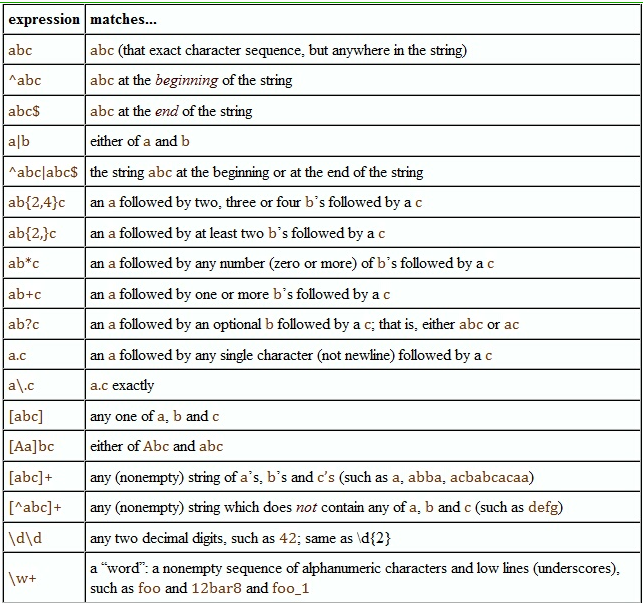
\includegraphics[width=3.6in]{/Users/fender/Dropbox/PCONS.DIR/IMG.DIR/regex.png}
\end{center}
\end{frame}

\begin{frame}[fragile]
\frametitle{Vectors - Character Vectors}
Character vectors also show up when we use the \textbf{list.files()} function to generate a list of files to be processed. 

For example let's say we have some files of the form 001.csv, 002.csv, .. 029.csv. Maybe we want to process some or all of them. First we have to generate a character vector containing the names. 
\small
\begin{verbatim}

files_to_be_read <- list.files(".","*.csv")

str(files_to_be_read)
 chr [1:29] "001.csv" "002.csv" "003.csv" "004.csv" "005.csv" 
            "006.csv" "007.csv" "008.csv" "009.csv" ...
            

\end{verbatim}
\end{frame}

%


\begin{frame}[fragile]
\frametitle{Vectors - DNA Strings}
DNA is a series of recurring letters. We can find patterns and ``motifs'' in stretches of DNA
strings. 
\scriptsize
\begin{verbatim}
dna <- c("A","A","C","G","A","C","C","C","G","G","A","T","G","A","C","T","G",
         "A","A","C")

# How many Gs are in the string ? 

grep("G",dna) # Extracts the elements numbers
[1] 4 9 10 13 17

dna[ grep("G",dna) ]
[1] "G" "G" "G" "G" "G"

# OR MORE SIMPLY
 
grep("G",dna, value = TRUE)
[1] "G" "G" "G" "G" "G"

length(grep("G",dna, value = TRUE)) # 5 occurrences of G
[1] 5
\end{verbatim}
\end{frame}

\begin{frame}[fragile]
\frametitle{Vectors - DNA Strings}
DNA is a series of recurring letters. We can find patterns and ``motifs'' in stretches of DNA
strings. 
\scriptsize
\begin{verbatim}
dna <- c("A","A","C","G","A","C","C","C","G","G","A","T","G","A","C","T","G",
         "A","A","C")

# How many Gs are in the string ? 

grep("G",dna) # Extracts the elements numbers
[1] 4 9 10 13 17

dna[ grep("G",dna) ]
[1] "G" "G" "G" "G" "G"

# OR MORE SIMPLY
 
grep("G",dna, value = TRUE)
[1] "G" "G" "G" "G" "G"

length(grep("G",dna, value = TRUE)) # 5 occurrences of G
[1] 5
\end{verbatim}
\end{frame}


\begin{frame}[fragile]
\frametitle{Vectors - DNA Strings}
\begin{itemize}
\item \textbf{We can use the sample function to simulate DNA strings} 
\end{itemize}
\footnotesize
\begin{verbatim}
set.seed(188)      # Allows us to reproduce the sample

( dna <- sample(c("A","C","G","T"),20,T) )
[1] "A" "A" "C" "G" "A" "C" "C" "C" "G" "G" "A" "T" "G" "A" "C" 
    "T" "G" "A" "A" "C"
\end{verbatim}

\normalsize
\begin{itemize}
\item \textbf{Find Gs or Cs in the simulated DNA string}
\end{itemize}

\footnotesize
\begin{verbatim}
grep("C|G",dna, value = TRUE)
[1] "G" "C" "G" "G" "C" "C"

length(grep("G|C",dna, value=T))
[1] 6
\end{verbatim}
\end{frame}

%

\begin{frame}[fragile]
\frametitle{Vectors - DNA Strings}
Let's look at some special cases that are important to know
\footnotesize
\begin{verbatim}
dna < c("A","A","C","G","A","C","C","C","G","G","A","T","G","A",
        "C","T","G","A","A","C")

my.str <- paste(dna,collapse="")
[1] "AACGACCCGGATGACTGAAC"

length(my.str)
[1] 1          # Not what you expected ?

my.str
[1] "AACGACCCGGATGACTGAAC"

rev(my.str)    # What's going on ?
[1] "AACGACCCGGATGACTGAAC"

str(my.str)    # Its now just a character string not a vector
chr "AACGACCCGGATGACTGAAC"
\end{verbatim}
\end{frame}

\begin{frame}[fragile]
\frametitle{Vectors - DNA Strings}
There are functions that work on character strings as opposed to character vectors
\footnotesize
\begin{verbatim}
my.str <- paste(dna,collapse="")
[1] "AACGACCCGGATGACTGAAC"

substr(my.str,1,1)
[1] "A"

substr(my.str,1,2)
[1] "AA"

substr(my.str,1,3)
[1] "AAC"

substr(my.str,1,4)
[1] "AACG"

gsub("TG","G",my.str)
[1] "AACGACCCGGAGACGAAC"
\end{verbatim}
\end{frame}

\begin{frame}[fragile]
\frametitle{Vectors - DNA Strings}
\small
\begin{verbatim}
my.str
[1] "AACGACCCGGATGACTGAAC"

substr(my.str,2,8)
[1] "ACGACCC"

substr(my.str,2,8) = "TTTTTTT"
my.str
[1] "ATTTTTTTGGATGACTGAAC"
\end{verbatim}
\end{frame}

\begin{frame}[fragile]
\frametitle{Vectors - DNA Strings}
\footnotesize
\begin{verbatim}
nchar(my.str)
[1] 20

for (ii in 1:nchar(my.str)) {
   cat(substr(my.str,ii,ii))
}
AACGACCCGGATGACTGAAC

for (ii in nchar(my.str):1) {
   cat(substr(my.str,ii,ii))
}
CAAGTCAGTAGGCCCAGCAA

# Recipe to get the "collapsed" string back into a vector with 
# separate elements for each letter

unlist(strsplit(my.str,""))
[1] "A" "A" "C" "G" "A" "C" "C" "C" "G" "G" "A" "T" "G" "A" "C" "T" "G" 
    "A" "A" "C"
\end{verbatim}
\end{frame}
%%%

%%% End of document
\end{document}
